\chapter{CDK2}
\label{cha:cdk2}

This chapter describes computational and experimental work to test a potential allosteric site on a protein important in cell cycle regulation, Cyclin-dependent kinase 2 (CDK2).
% Change this to section ref
This allosteric site was predicted by ExProSE in Chapter~\ref{cha:exprose}.
A virtual screen of small molecules was carried out against the pocket.
Selected molecules were purchased and tested using two experimental assays to see if they could inhibit the interaction between CDK2 and Cyclin A.


\section{Materials and Methods}
\label{sec:cdk2_methods}

Bioinformatics resources generally had 3PXF as input.


\subsection{Virtual screening}

The receptor and ligands are prepared in line with the AutoDock Vina documentation.

ChemMine clustering used binning clustering at a similarity cutoff of 0.5.
The highest ranked by docking scores was retained in each case.

The selected structure has the maximum sum of two distances across the opening of the pocket: the distance between atom OH on residue TYR180 and atom NH1 on ARG150, and the distance between atom OG on residue SER188 and atom O on THR165.
This struture is energy minimised as described in Section~\ref{sec:exprose_methods} to remove any violations of stereochemistry.


\subsection{Reagents and compounds}

The buffers and media used were as follows:
\begin{itemize}
\item Auto-induction media: 10 g\\L tryptone, 5 g\\L yeast extract, 5052, NPS, 1 M MgSO$_{4}$, Ampicillin.
\item LB broth: 10 g\\L tryptone, 5 g\\L yeast extract, 10 g\\L NaCl.
\item Lysis buffer: 50 mM HEPES pH ?, 150 mM NaCl, 10 mM MgCl$_{2}$, 2 mM DTT, 1 mM EGTA, Triton.
\item Tris pH 8 buffer: 100 mM Tris-HCl pH 8.0, 150 mM NaCl, 10 mM MgCl$_{2}$.
\item TBS-T buffer: 50 mM Tris-HCl pH 7.5, 150 mM NaCl, 0.1\% Tween 20 (?).
\item Transfer buffer: 20\% methanol, 190 mM glycine, 25 mM Tris.
\end{itemize}


\subsection{Purification of Cyclin A}

The plasmid for His-tagged Cyclin A (residues ) was transformed into \textit{E. coli} Tuner cells.
Various conditions for growth were tried (see results).
The final conditions used were growth of cultures at 37$^{\circ}$C until optical density in auto-induction media, then incubated at 18$^{\circ}$C for 40 hours.
Cells were harvested by centrifugation (10 min at 5,000 rpm).
Harvested cells were resuspended in lysis buffer with 0.5 mg ml$^{-1}$ (?) lysozyme.
After sonication and centrifugation (30 min at 16,000 rpm) the supernatant was incubated on Sepharose (?) beads for 1 hour.
After washing the beads Cyclin A was eluted with imidazole and stored at -20$^{\circ}$C (?) in 50\% glycerol.
% Amounts and concentration produced?


\subsection{TR-FRET assay}

CDK2 was labelled with Cy5 dye...
CDK2 (10 mg/ml) in 0.1 M NaHCO$_{3}$ was incubated overnight with NHS ester dye in anhydrous DMF.
Excess dye was removed by gel filtration.

For the TR-FRET CDK2 titration a 392 (?) well plate was used.
Each well contained 1 nM Cyclin A-His, 1 nM Eu-anti-His antibody and CDK2 at various concentrations in 50\% glycerol/50\% phosphate buffer.
A control with no CDK2 and 10 CDK2 concentrations were used, with a highest concentration of 1 \textmu M and each well being a three-fold dilution for a lowest concentration of 50 pM.
The plate was incubated for 1 hour and centrifuged at 800 rpm.
... plate reader was used to read the plate.
20 (?) repeats were taken for each reading.


\subsection{Binding assay}
% More specific - immunoblotting assay?

Wild-type CDK2 was previously prepared in the lab.
His-tagged Cyclin A (75 nM) was incubated on Sepharose fast flow beads (?) in buffer X with 12\% DMSO.
CDK2 was added (8 nM) along with compounds in 5 concentrations: 0 M control, 8 \textmu M, 40 \textmu M, 200 \textmu M and 1 mM.
After incubation for 1 hour the beads were washed with buffer X and heated in gel-loading dye at 100$^{\circ}$C for 10 minutes to release bound protein.
The proteins in the supernatant were separated by SDS-PAGE and transferred to a nitrocellulose membrane by electroblotting in transfer buffer for 1 hour at 100 V.
The membrane was incubated for 15 minutes in TBS-T buffer with 1.5\% skimmed milk powder.
The primary antibody, CDK2 rabbit polyclonal antibody ( M) was added and the membrane incubated overnight at 4$^{\circ}$C.
After washing with TBS-T the secondary antibody was added ( M) and incubation for 1 hour carried out.
The membrane was washed with TBS-T and imaged by adding ... and 1 s exposure.
% Check with other papers that do this


\section{Results}
\label{sec:cdk2_results}

Having predicted a new allosteric site on CDK2 using ExProSE, we seeked to test experimentally whether it was in fact an allosteric site.
See Section~\ref{sec:exprose_results} and Figure~\ref{fig:cdk2} for a description of how ExProSE predicts pocket 3, henceforth referred to as the pocket of interest, as being allosteric.
This pocket is not open in the apo CDK2 structure (PDB ID 1HCL) or in the Cyclin A-bound structure (PDB ID 1FIN).
In the Cyclin A-bound structure there is in fact a protrusion instead of a pocket opening, suggesting that a small molecule would not be able to bind the pocket at the same time as Cyclin A is bound to CDK2 (?).
The pocket is open but small (45 \AA$^{3}$ in LIGSITE\textsuperscript{\it cs}) in the structure with two ANS molecules bound in the known allosteric site (PDB ID 3PXF).
It is a similar shape in the structure with two ANS molecules and the active site inhibitor staurosporine (PDB ID 4EZ7).
This structure also has the crystallisation artefact ethanediol crystallised at the pocket of interest, implying that binding there is possible.
A structure with ethanediol bound at the ANS site and an active site inhibitor (PDB ID 4EZ3) appears to have the pocket slightly open.
This furthers the suggestion that (conf selection and inactive state) the inactive state caused by binding at the ANS site is linked to the presence of the pocket.
The idea is that by stabilising the pocket of interest the inactive state is favoured and activation by Cyclin A cannot occur.
The hope is that the pocket of interest can accommodate a small molecule ligand, and potentially that it can open further to present more binding interactions.
One risk of targeting this site is that the pocket is small, meaning a limited number of interactions can be made with a ligand.
The pocket is also only available in some states, meaning that there may be an energetic cost to stabilising it.
Off site binding may also be a problem - the ATP-binding site and ANS allosteric site present large pockets on CDK2 and small molecules may preferentially bind to these.
% Given that I mention this should mention cross-docking?
For example, scanning the surface for binding hotspots using FTMap \cite{Kozakov2015} does not predict the pocket of interest as a binding site.
The Fragment Hotspot Map \cite{Radoux2016} samples the protein surface with molecular probes to find fragment binding hotspots.
Applying the Fragment Hotspot Map to CDK2 does not reveal the pocket of interest as a fragment binding site in the default map.
However adjusting the score cutoff does show there is some ability for fragment to bind to the pocket.

ResiCon calculates dynamic regions in proteins by considering contacts between residues \cite{Dziubinski2016}.
ResiCon was run on CDK2.
The pocket of interest seems to be on the edge of dynamic domains across a variety of given numbers of domain outputs, including the default result of two domains.
% Possibly this in the figure, may need to split the figure up
This indicates that the site could have the ability to cause structural rearrangement in distal parts of the protein by acting as a hinge that responds to ligand binding.
This is further evidenced by examining CDK2 using the DynOmics server \cite{Li2017}.
Residue that are close to the pocket of interest, such as ASP127 in the pocket, are predicted to be hinge residues that control the two slowest normal modes.
% Possibly this in figure too

%In fact, the CoDNaS database \cite{Monzon2013} (not in Mendeley) showing conformational diversity of native states in proteins shows that the structures with PDB ID 3PXF and 4EZ7 are in the same...
% Not too strong, RMSD could probably show this - RMSD values anywhere here?

There are 371 structures of human CDK2 present in the PDB.
Of these, x are bound to Cyclin proteins (A and E separate?), including 17 to non-human Cyclins.
x of the 371 are bound to ATP-binding site inhibitors. % Use Proteopedia to help here
x have binding at the ANS allosteric binding site \cite{Betzi2011}? % Check related strucs for number

PDB - n strucs, nothing bound apart from EDO in 3QQH/4EZ7.
Talk about there being an internal cavity in other strucs?
PDBFlex database (and written)


% Make sure all parts of this are referenced from main text
% What about apo (1HCL) or Cyclin A-bound (1FIN)?
\begin{figure}
\centering

%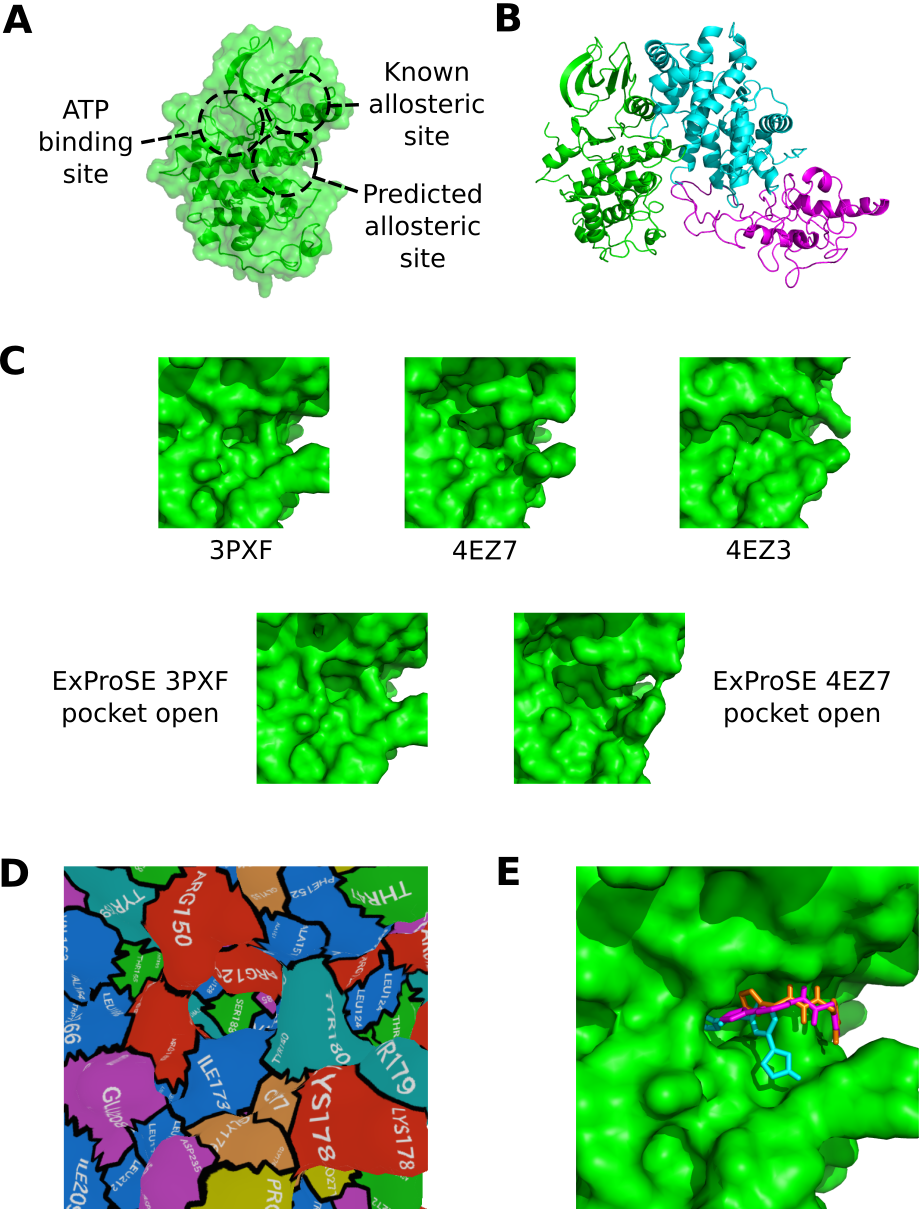
\includegraphics[width=\textwidth]{figures/cdk2_structure}

\caption{Structure and screening of CDK2.
(A) The structure of CDK2 (PDB ID 1HCL) with colours, including existing allosteric site, active site, T loop, C-helix...
(B) The CDK2-Cyclin A complex required for CDK2 activation.
The crystallised complex (PDB ID 1FIN) is shown with CDK2 in green and the crystallised portion of Cyclin A in cyan.
The whole Cyclin A sequence was modelled using Phyre2 \cite{Kelley2015} and aligned to the above complex and the ab initio modelled region (with no structural templates) is shown in magenta.
Part of this region potentially interacts with CDK2.
(C) The pocket of interest on CDK2 shown in various structures.
This is pocket 3 from Figure~\ref{fig:cdk2}.
The structures shown are three crystal structures with the PDB IDs given, and two structures with the pocket open generated using ExProSE from the structures indicated.
(D) Residues displayed around the pocket of interest using SurfStamp (\url{https://yamule.github.io/SurfStamp-public}). % http://process.sakura.ne.jp/surfstamp/viewer/test.cgi?pdbid=3PXF
The orientation is the same as in C.
(E) Example docking poses of screened compounds using AutoDock Vina on the structure with PDB ID 3PXF.
Shown are the lowest energy poses for compound A (magenta), B (cyan) and C (orange) from Table~\ref{tab:enamine_compounds}.}

\label{fig:cdk2_structure}
\end{figure}


\subsection{Virtual screening}

A virtual screening strategy was carried out to predict compounds that bind to the pocket of interest.
ZINC is a free database of commercially-available compounds for virtual screening \cite{Sterling2015}.
The ZINC12 LeadsNow subset contains over 3 million lead-like molecules in stock at chosen suppliers.
Lead-like molecules have a molecular weight between 250 and 350, an octanol-water partition coefficient not greater than 3.5 and no more than 7 rotatable bonds.
These criteria give smaller and more x molecules than those that would conventionally end up being drugs.
This is because at the hit stage the priority is finding effective scaffolds with high affinity per atom (ligand efficiency).
Elaboration of the structure with further functional groups generally occurs later and would usually result in the addition of chemical groups, raising the molecular weight.
The LeadsNow subset is clustered using a 90\% Tanimoto cutoff as described at \url{http://zinc.docking.org} to get a representative subset of $\sim$250,000 compounds.
These compounds are docked using AutoDock Vina \cite{Trott2010} to the pocket of interest in the ANS-bound structure, PDB ID 3PXF.
AutoDock Vina...
% Sidechains allowed to move?
Examples of docking poses can be seen in Figure~\ref{fig:cdk2_structure}E.
The top 2,000 structures by affinity score from this screen were retained for further docking studies.
This was due to the computational cost of virtual screening - the score from AutoDock Vina on the ANS-bound structure was used to eliminate most compounds and the remaining compounds were taken forward for further studies.
The 2,000 retained molecules were docked using AutoDock Vina and DOCK \cite{Allen2015} onto four structures:
\begin{itemize}
\item The ANS-bound structure, PDB ID 3PXF.
\item The ANS-bound structure with the active site inhibitor staurosporine, PDB ID 4EZ7.
\item A structure selected from an ensemble of structures generated from (1) using ExProSE.
The structure selected is the one with the pocket of interest most open.
\item The same as (3) but the ensemble is generated using ExProSE from (2).
\end{itemize}
The structure of the pocket of interest in each of these structures is shown in Figure~\ref{fig:cdk2_structure}C.
Docking to multiple structures means the compounds are scored in multiple conformations of the binding site, which is an approximation of ensemble docking.
This is important in general to take into account the flexibility of binding pockets, and especially important for this pocket as it is a flexible pocket not present in all structures.
Using two different docking algorithms, AutoDock Vina and DOCK, provides two different scores for each structure and goes some way to reducing the inaccuracies of virtual screening.
Compounds were in general better scored for structures (3) and (4), those with the pocket of interest open.
This is to be expected as a larger pocket presents more opportunities for interactions with the ligand.
% Mention cross-docking? Possibly not


\subsection{Compound selection}

Compounds were ranked by the average of the 8 scores from the above docking (4 structures, 2 docking methods).
In addition to the lead-like properties described previously, compounds were further filtered to remove compounds that would potentially give erroneous assay results.
Compounds violating various criteria set out by the SwissADME server for assessing medicinal chemistry friendliness \cite{Daina2017}, such as properties of pan-assay interference compounds \cite{Baell2014}, were removed.
Compounds marked as not having benign chemical functionality in ZINC12 were also removed.
Although compounds were clustered by ZINC12 to remove similar compounds, some compounds were relatively similar to each other on visual inspection.
Compounds were hence removed by similarity in ChemMine \cite{Backman2011}.
The top 20 ranked compounds remaining that were available from Enamine (\url{http://www.enamine.net}) were purchased and taken forward for experimental testing.
The structures of the compounds are shown in Figure~\ref{fig:compound_structures}.
Docking scores and compound IDs are shown in Table~\ref{tab:enamine_compounds}.
None of these are found as ligands in the PDB.


\begin{sidewaystable}
\centering

\begin{small}
% Table generated by Excel2LaTeX from sheet 'compounds'
\begin{tabular}{lllrrrrrrrrr}
\hline
      &       &       &       & \multicolumn{4}{c}{\textbf{AutoDock Vina best energy / units?}} & \multicolumn{4}{c}{\textbf{DOCK best grid score / units?}} \\
\textbf{Compound ID} & \textbf{ZINC12 ID} & \textbf{Enamine ID} & \multicolumn{1}{l}{\textbf{Molecular weight (g/mol)}} & \multicolumn{1}{l}{\textbf{A}} & \multicolumn{1}{l}{\textbf{B}} & \multicolumn{1}{l}{\textbf{C}} & \multicolumn{1}{l}{\textbf{D}} & \multicolumn{1}{l}{\textbf{A}} & \multicolumn{1}{l}{\textbf{B}} & \multicolumn{1}{l}{\textbf{C}} & \multicolumn{1}{l}{\textbf{D}} \\
\hline
A     & ZINC06731189 & Z28083007   & 279.3 & -7.1  & -8.1  & -7.6  & -7.4  & -37.3 & -40.0 & -40.8 & -35.1 \\
B     & ZINC29799246 & Z2241108787 & 281.3 & -7.4  & -7.9  & -7.9  & -7.7  & -31.2 & -38.9 & -39.7 & -32.4 \\
C     & ZINC58182552 & Z953947716  & 273.3 & -7.2  & -7.4  & -7.8  & -7.4  & -32.8 & -39.3 & -41.5 & -36.0 \\
D     & ZINC03275010 & Z56813876   & 280.3 & -7.3  & -7.3  & -7.3  & -7.7  & -36.5 & -39.2 & -40.6 & -36.3 \\
E     & ZINC25129280 & Z125831222  & 281.3 & -7.3  & -7.8  & -7.1  & -7.5  & -32.8 & -41.2 & -39.9 & -38.8 \\
F     & ZINC97022380 & Z1537396696 & 280.3 & -7.7  & -7.6  & -7.4  & -7.8  & -35.0 & -37.0 & -38.2 & -32.6 \\
G     & ZINC84057181 & Z1367181624 & 280.3 & -7.2  & -7.8  & -7.9  & -7.4  & -30.9 & -37.8 & -35.5 & -37.1 \\
H     & ZINC30691564 & Z383528790  & 281.3 & -7.2  & -7.2  & -7.8  & -7.8  & -35.3 & -35.3 & -41.6 & -33.8 \\
I     & ZINC36390489 & Z381531134  & 279.3 & -7.6  & -7.3  & -7.5  & -7.5  & -31.2 & -39.3 & -37.5 & -34.7 \\
J     & ZINC89878745 & Z1159552572 & 279.3 & -7.0  & -8.0  & -8.3  & -7.2  & -37.3 & -38.3 & -38.9 & -32.5 \\
K     & ZINC12812500 & Z220404550  & 279.3 & -7.0  & -7.9  & -7.5  & -7.7  & -31.8 & -38.1 & -39.0 & -34.6 \\
L     & ZINC75147268 & Z1262428103 & 281.3 & -7.3  & -7.8  & -7.8  & -7.5  & -28.8 & -36.0 & -37.6 & -34.4 \\
M     & ZINC71914433 & Z1232176487 & 274.3 & -7.0  & -7.4  & -7.4  & -7.5  & -36.2 & -37.6 & -40.2 & -35.7 \\
N     & ZINC72288573 & Z1229931451 & 268.3 & -7.7  & -7.8  & -7.9  & -7.4  & -29.4 & -36.2 & -33.3 & -34.1 \\
O     & ZINC69453509 & Z1030096350 & 287.4 & -7.2  & -7.6  & -7.1  & -7.7  & -33.9 & -40.5 & -33.1 & -35.8 \\
P     & ZINC79097391 & Z1408168262 & 281.3 & -7.0  & -7.6  & -7.6  & -7.3  & -33.7 & -38.5 & -37.5 & -33.8 \\
Q     & ZINC16497227 & Z66926805   & 280.3 & -6.9  & -7.4  & -7.8  & -7.9  & -29.2 & -38.8 & -40.0 & -33.5 \\
R     & ZINC23143433 & Z352550190  & 271.3 & -7.5  & -7.3  & -6.9  & -7.1  & -32.5 & -39.6 & -38.4 & -36.2 \\
S     & ZINC89858262 & Z1162482939 & 273.3 & -7.2  & -7.3  & -8.3  & -7.4  & -23.9 & -35.1 & -39.6 & -36.2 \\
T     & ZINC69369685 & Z1097406485 & 272.3 & -7.2  & -7.1  & -7.0  & -7.1  & -37.0 & -40.6 & -43.1 & -35.6 \\
\hline
\end{tabular}
\end{small}
% Average of scores?

\caption{Selected compounds to screen experimentally against a potential allosteric site on CDK2.
ZINC12 ID is the ID in the ZINC12 database (\url{http://zinc.docking.org/}).
Enamine ID is the ID at Enamine Ltd (\url{http://www.enamine.net}).
The AutoDock Vina best energy and DOCK best grid score are shown for each ligand docked to four structures:
(A) 3PXF,
(B) 4EZ7,
(C) ExProSE pocket open structure from 3PXF,
(D) ExProSE pocket open structure from 4EZ7.}
% Or refer to main text for structure information?

\label{tab:enamine_compounds}
\end{sidewaystable}


\begin{figure}
\centering

%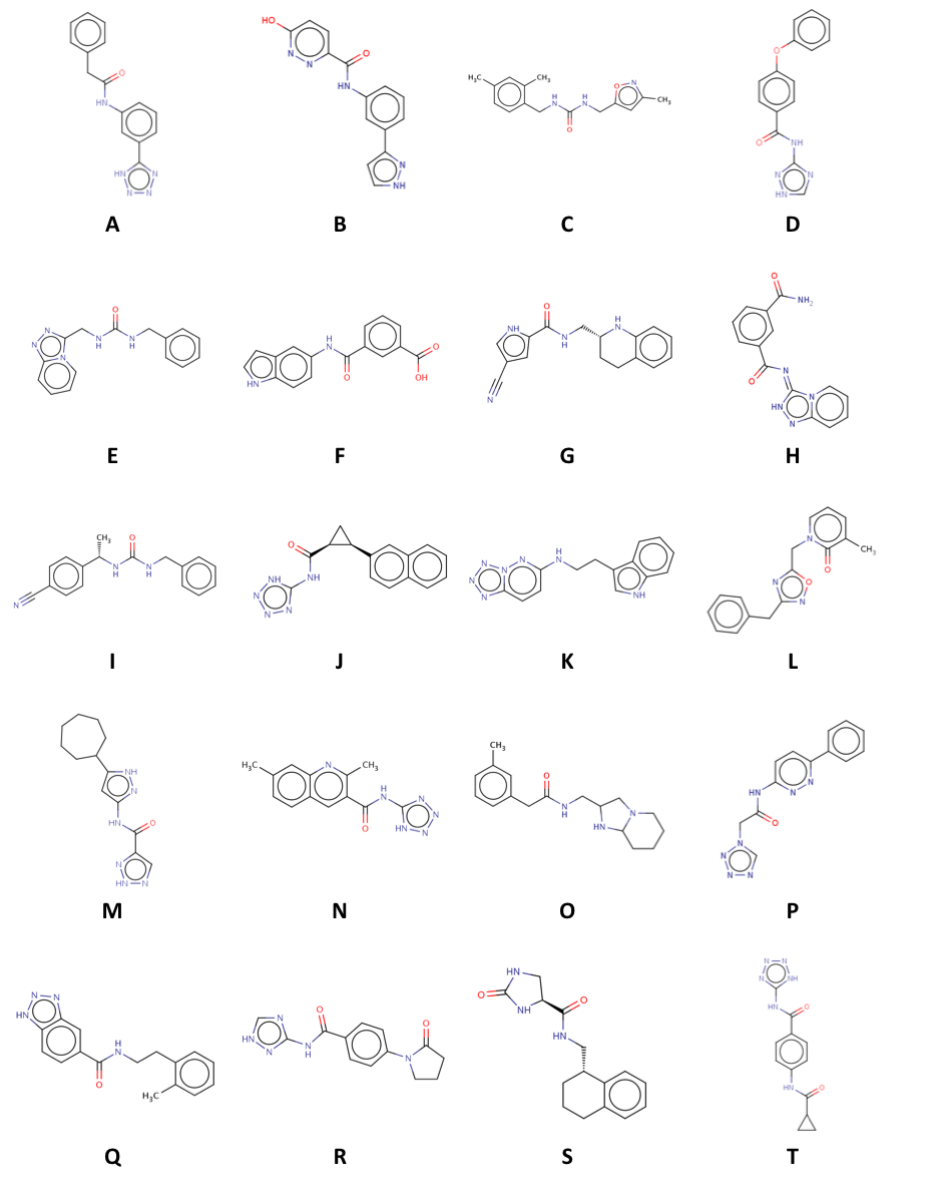
\includegraphics[width=\textwidth]{figures/compound_structures}

\caption{Chemical structures of selected compounds to screen experimentally against a potential allosteric site on CDK2.
The compounds are labelled as in Table~\ref{tab:enamine_compounds}.
Images generated using \url{http://cdb.ics.uci.edu/cgibin/Smi2DepictWeb.py}.}

\label{fig:compound_structures}
\end{figure}


\subsection{Experimental aims}

The main aim of the experimental work was to screen the purchased compounds using the TR-FRET assay.
This popular assay for drug discovery research is the combination of time-resolved fluorometry with F\"{o}rster resonance energy transfer (FRET).
FRET involves two fluorophores, a donor and an acceptor.
Figure~\ref{fig:tr_fret}A outlines the principles of a TR-FRET assay.

% Excitation of the donor by an energy source (e.g. flash lamp or laser) produces an energy transfer to the acceptor if the two are within a given proximity to each other. The acceptor in turn emits light at its characteristic wavelength.

A time delay between excitation and measurement means measurement occurs after the timescale of background fluorescence.
The long emission time of the donor fluorophore means a signal is obtained after the time delay.


\subsection{Purification of Cyclin A}
% Describe GST and His tags

% Mention the construct is not all of Cyclin A
There are x surface-exposed cysteine residues on Cyclin A (construct?).
In order to improve the TR-FRET signal it would be beneficial to have a single surface-exposed cysteine that could be labelled with Cy5 dye.
Hence, initial purification was attempted for Cyclin A-GST (mut).
The GST tag allowed selective separation of the protein during purification.
The His tag could not be used as this was going to be present on CDK2 to bind the donor fluorophore.
Purification of Cyclin A-GST (mut) resulted in low quantities of soluble protein (x mg from y L media) and purity was low, as shown in Figure~\ref{fig:purification}A.
Different purification strategies including varying the media, incubation temperature and incubation times were attempted.

The difficulty of purifying this Cyclin A mutant led us to try purification of the wild-type Cyclin A-GST (with truncation though).
This purified more readily than the mutant, as shown in Figure~\ref{fig:purification}A.
x mg from y L media, which is still low...
This could be because the x mutation destabilises the protein, increasing its tendency to aggregate.
% Here or discussion?
However concentration of the protein to higher concentrations using spin filtration led to loss of the protein.
This, along with the low yield, suggests that Cyclin A-GST is unstable and has a tendency to aggregate and become insoluble.

Due to the difficulty of purifying Cyclin A-GST, a change was made to the experimental strategy.
The donor and acceptor fluorophores were switched so that the Eu anti-His antibody was targeted at Cyclin A and CDK2 was dyed with Cy5 dye - see Figure~\ref{fig:tr_fret}B.
This required purification of Cyclin A-His.
This purification proved considerably more successful than Cyclin A-GST, with x mg produced from y L media - see Figure~\ref{fig:purification}C.
This indicates that the large GST tag may disrupt the stability or folding of Cyclin A.
Purified Cyclin A-His was taken forward for the TR-FRET assay.

\begin{figure}
\centering

%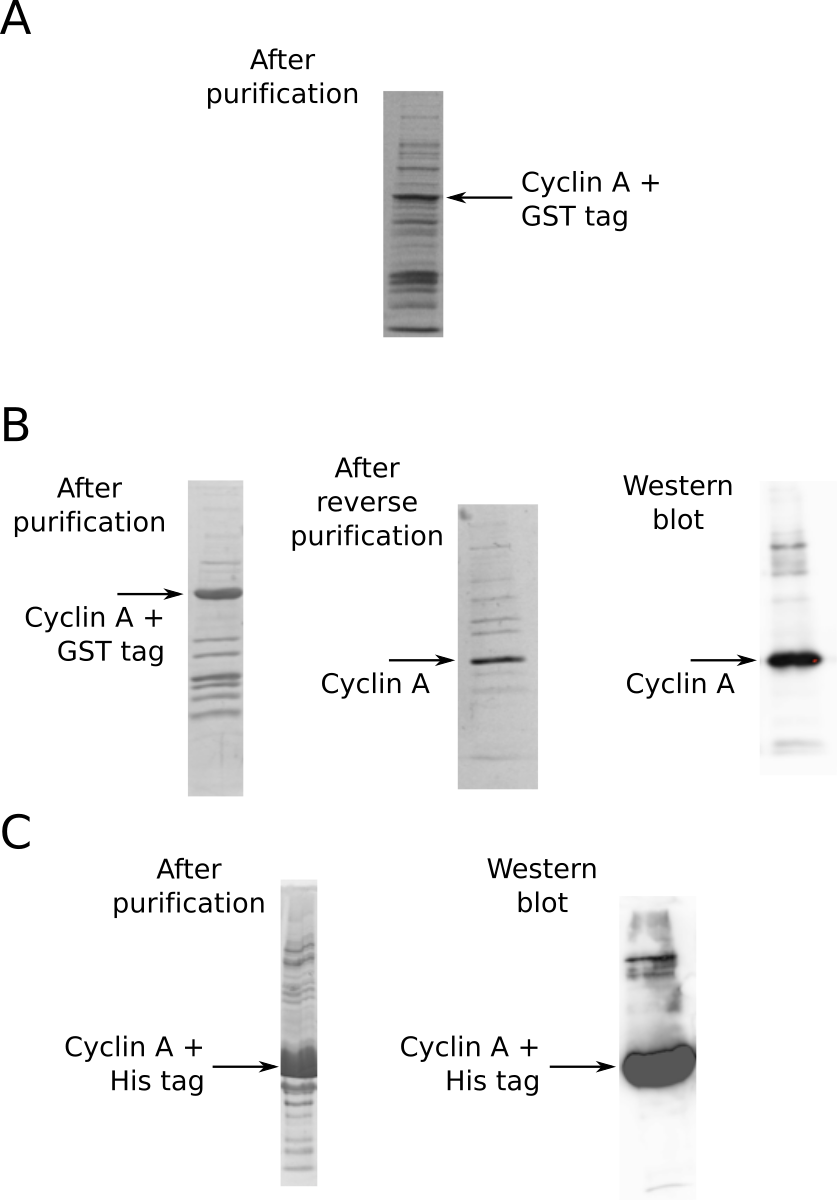
\includegraphics[width=\textwidth]{figures/purification/purification}

\caption{SDS-PAGE results for purification of Cyclin A.
(A) Purification of Cyclin A-GST single cysteine mutant (mut).
% Gels for other conditions?
% Pellet gel?
(B) Purification of Cyclin A-GST.
(C) Purification of Cyclin A-His.}

\label{fig:purification}
\end{figure}


\subsection{TR-FRET}

CDK2 prepared previously in the lab was labelled with Cy5 dye (see fig for reaction?).
The TR-FRET assay was tested using a titration of CDK2 with constant Cyclin A and donor fluorophore.
An increase in signal with increasing CDK2 concentration would be expected.
Figure~\ref{fig:tr_fret}B shows the result of this titration.
Whilst there is a higher signal at higher CDK2 concentrations, this trend is also present for the control of Cyclin A-GST.
Cyclin A-GST lacks the His tag required to bind to the donor fluorophore so should not lead to a TR-FRET signal.
This indicates that the increased signal with CDK2 concentration is likely due to excess, unbound Cy5 dye in the CDK2 solution.
Time constraints meant that a further gel filtration could not be carried out to remove this unbound dye.
The high background signal would means the screen would not be effective at finding compounds that inhibit the Cyclin A-CDK2 interaction, so the compounds were not put through the TR-FRET screen.

\begin{figure}
\centering

%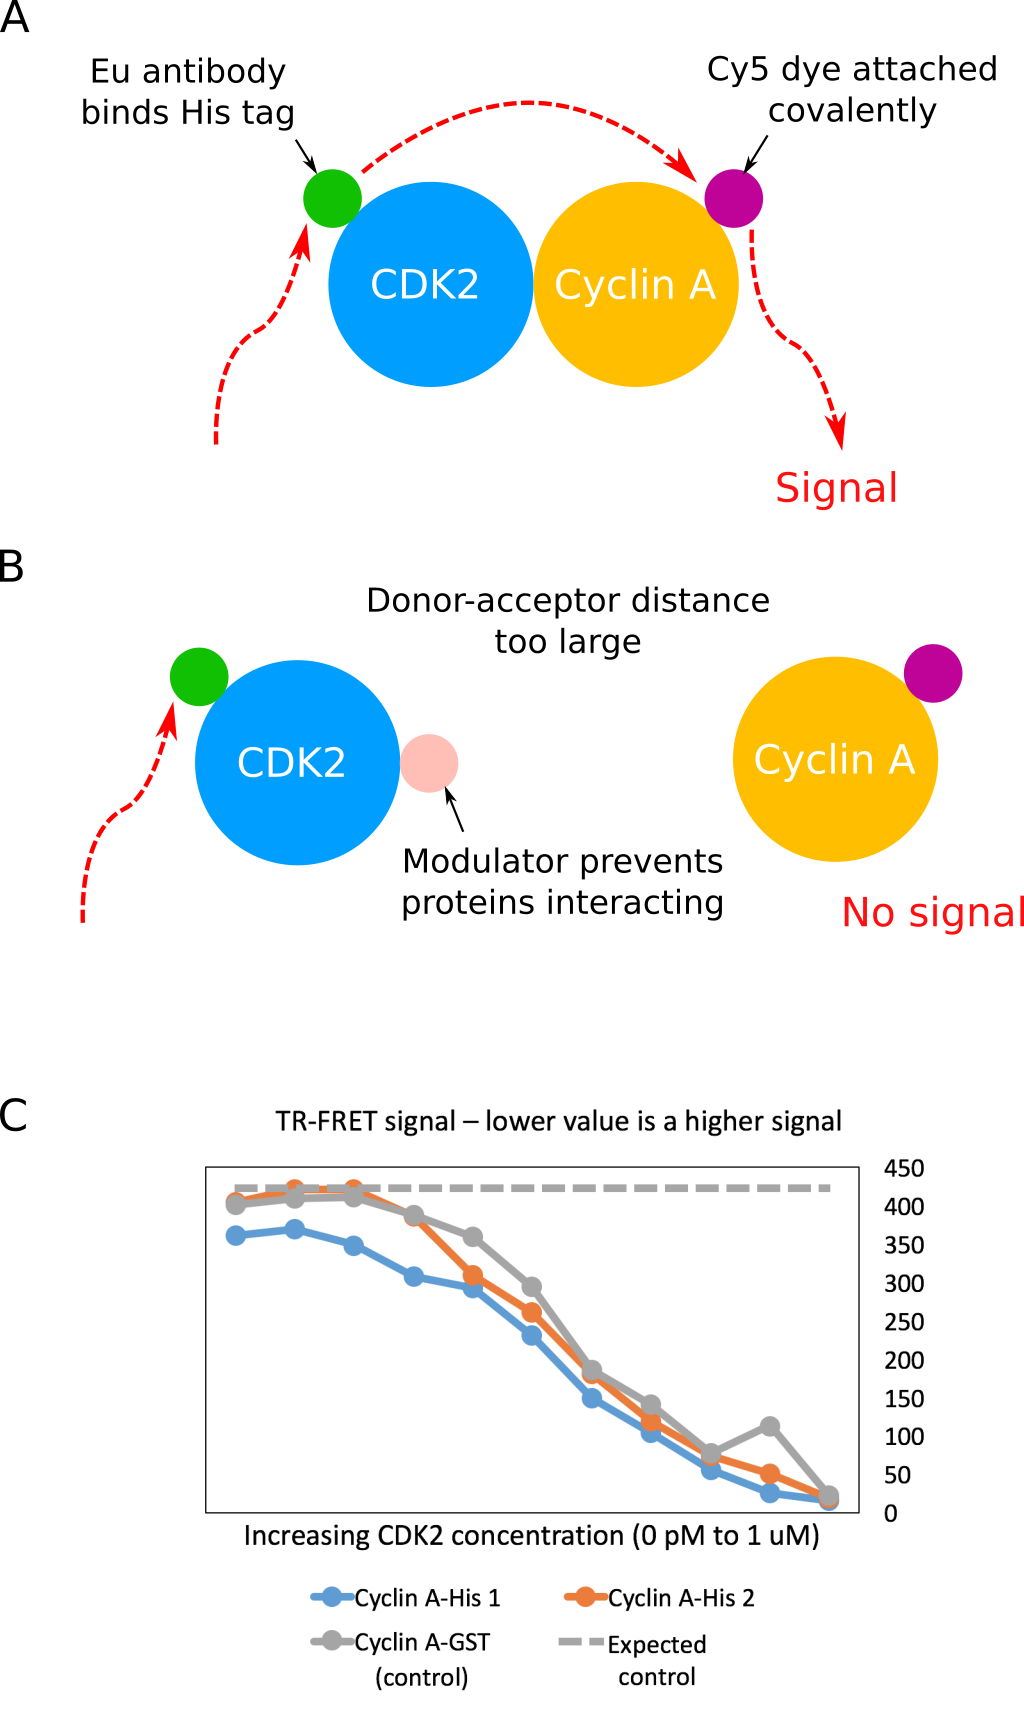
\includegraphics[width=\textwidth]{figures/tr_fret}

\caption{(A) The principle of the TR-FRET assay used.
One protein in the binding pair is covalently-bound to Cy5 dye (the acceptor fluorophore).
The other protein is targeted with an antibody containing the lanthanide Eu (the donor fluorophore).
Light is shone at the excitation wavelength of the donor fluorophore.
This emits at the excitation wavelength of the acceptor fluorophore.
After a delay to allow background emission to recede, emission from the acceptor fluorophore is measured.
If a modulator prevents the proteins interacting, emission from the donor to the acceptor fluorophore is not possible and there is no signal.
(B) After difficulty purifying Cyclin A-GST, the strategy was switched so Cyclin A-His binds the Eu antibody and CDK2 is labelled with the dye.
% NHS-ester reaction as below?
% https://www.thermofisher.com/uk/en/home/life-science/protein-biology/protein-biology-learning-center/protein-biology-resource-library/pierce-protein-methods/amine-reactive-crosslinker-chemistry.html
(C) Results of a CDK2 titration TR-FRET assay.}
% Different figure?

\label{fig:tr_fret}
\end{figure}


\subsection{Binding assay}

A binding assay was carried out to test whether the compounds could inhibit the CDK2-Cyclin A interaction.
Cyclin A-His and CDK2 were incubated with beads that selectively bind His tags.
After washing the beads to remove unbound protein only Cyclin A and proteins bound to it should remain.
In the absence of a PPI inhibitor a signal for CDK2 would be expected in immunoblotting as CDK2 binds to Cyclin A.
This signal would be expected to disappear in the presence of a modulator that prevented the interaction.

The binding assay results can be seen in Figure~\ref{fig:binding_assay} for the 12 compounds it was carried out on.
A significant problem with the assay was binding of CDK2 to the beads despite the lack of a His tag on CDK2.
This gave a significant background signal and means that a signal from the compounds would be hard to distinguish from the background.
However, some compounds do appear to remove the CDK2 signal at high concentrations.
Compound D at 200 \textmu M and 1 mM, and compound J at 1 m, cause the CDK2 signal to decrease.
As the expected background is high this is probably due to solubility issues of those compounds at high concentrations...
% Assay not very quanititative anyway
% Fluorescent also tried (gel)

\begin{figure}
\centering

%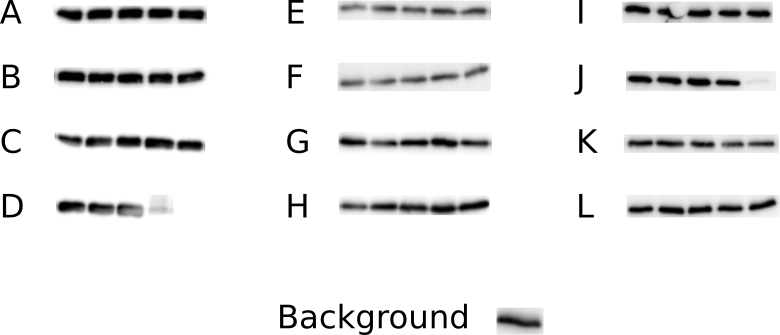
\includegraphics[width=\textwidth]{figures/binding_assay}

\caption{(A) Binding assay results for the 12 compounds tested.
The five bands represent increasing compound concentrations from left to right: 0 M control, 8 \textmu M, 40 \textmu M, 200 \textmu M and 1 mM.
The strength of the band represents the presence of CDK2.
The background signal, in the absence of Cyclin A, is also shown.
This shows non-specific binding of CDK2 to the beads and indicates that a signal in the assay would be hard to distinguish from the background.}

\label{fig:binding_assay}
\end{figure}


\section{Discussion}

% Difficulty of purifying Cyclin A, due to flexible structure?, also GST may affect folding, ref to lack of crystal structure for certain region (run Disopred to check disorder?).
The difficulty of purifying Cyclin A is likely due to the propensity of the protein to aggregate.
As shown in Figure~\ref{fig:cdk2_structure}B the crystal structure of the CDK2-Cyclin A complex has only been found for part of the structure.
Cyclin A alone has not been crystallised??
The presence of the GST tag made Cyclin A purification considerably more difficult than the His tag.
This could be due to the large GST segment causing problems with folding leading to aggregation in the fusion protein.
% Check the paper, was it hard to crystallise?

Though time constraints meant that no more experiments could be carried out, there are a number of other tests that could be done.
Primarily this would involve further work on the TR-FRET and binding assays to reduce background signal and allow the compounds to be screened.
Other tests that could be carried out include:

\begin{itemize}
\item X-ray crystallography: hit compounds in other screens could be incubated with CDK2 and an attempt could be made at obtaining a crystal.
If successful this would indicate where the compound binds on CDK2, and show conformational changes due to binding.
It would also facilitate further computational studies on the new structure.
\item Anti-proliferation assay: adding a compound to cancer cells should stop cell proliferation if the compound completely inhibits CDK2-Cyclin A interaction.
This assay does not indicate that the compound is specific to the CDK2-Cyclin A interaction however, as any effect that prevents proliferation will appear in the assay.
\item Kinase assay: Cyclin A is required for the activation, and hence kinase activity, of CDK2 \cite{Jeffrey1995}.
Assays that measure the kinase activity in the presence of the compounds indicate whether they are able to prevent CDK2 activation by Cyclin A.
% Check Cyclin A/E differences
\item Mutagenesis: a mutation in the putative binding site of a compound will likely disrupt binding.
If inhibition occurs for the wild-type CDK2 but not for a mutant with a mutation, this gives evidence that the mutation site is the binding site.
% Or disrupts communication
This assumes that the mutation has no other effect on the structure, such as destabilisation.
\item Thermal shift assay: circular dichroism can be used to measure the unfolding of a protein by observing changes in plane-polarised light. % near/far?
If a compound bound to CDK2 it may change the temperature at which the protein unfolds.
\item Surface plasmon resonance:
\item Cyclin E studies: \cite{}
\end{itemize}
